% -*- root: 00-main.tex -*-
\section*{Results}
\label{sec:results}

\subsection*{Proof of concept on digital phantoms}
\label{sec:results_phantom}
Using a simplified subset of the experimental instrumentation described in section
  \nameref{sec:experiments_evaluation}, we collected quantitative results on the digital
  phantoms.
To warp the simulated datasets, we randomly generated 150 different realizations of
  the distortion $U_{true}$.
Smoothness is introduced using two levels of B-Spline functions, with control points evenly
  located in isotropic grids covering the full extent of the phantom.
The first level had $50.5mm$ of separation between control points and the second $25.25mm$.
The rationale behind this choice is producing large deformations on the contours with
  the first level, and matching the properties of susceptibility-derived distortions
  as previously reported by \cite{irfanoglu_susceptibility_2011} with the finer grid.
Invertibility of $U_{true}$ is ensured by controlling the maximum displacement at each
  level ($20.2mm$ and $10.1mm$ respectively) as studied in \citep{rueckert_diffeomorphic_2006}.

A total of 1200 registration experiments (4 phantom types $\times$ 150 random warpings
  $\times$ 2 resolutions) were run.
Parameter settings of every processing step in the experiments are made available along with
  the source code.
For each registration, the averaged Hausdorff distance (see \nameref{sec:experiments_evaluation})
  of the inner and the outer surfaces was computed.
The results showed a consistent and high accuracy, below voxel resolution.
\autoref{fig:phantom} (block C) presents the box plots by model type corresponding
  to the two sets of resolutions of generated phantoms.
To support that the misregistration errors averaged per experiment was significantly
  under the resolution of the target image, we proceeded as follows.
First, we confirmed that the error distributions were skewed using a Shapiro-Wilk test of
  normality.
All the distributions of errors under test (4 phantom types $\times$ 2 resolutions) resulted
  non-normal with $p<0.001$.
Consequently, we used the non-parametric Wilcoxon signed-rank test along with Bonferroni
  correction for multiple comparisons ($N=150$).
Averaged errors resulted significantly lower than voxel resolution with $p < (0.001 / 150)$
  for all the tests (4 phantom types $\times$ 2 resolutions).
Since statistical tests may not be conclusive enough, we also computed the confidence intervals
  (\autoref{tab:ci_phantom}).


\begin{table}
		\centering
		\footnotesize
    \begin{tabular}{llcc}
    Type      & Low-res.  & Hi-res. \\
    \hline
    ``gyrus'' & 0.58-0.60 & 0.18-0.36 \\
    ``L''     & 0.67-0.73 & 0.35-0.39 \\
    ``ball''  & 0.66-0.73 & 0.32-0.41 \\
    ``box''   & 0.68-0.71 & 0.35-0.39 \\
    \hline
    \end{tabular}
    \caption{All the 95\% confidence intervals (CI) were below the corresponding
      half-voxel resolution in all the phantom types.
    CIs reported in this table were computed using bootstrapping of $10^4$ samples,
      for each phantom type and resolution.
    Taking into account the non-normal distribution of errors, we used the median as location
  		statistic.}\label{tab:ci_phantom}
\end{table}

\subsection*{Correction of distortions on real datasets}\label{sec:results_hcp}

\paragraph*{Assessing the segmentation model}\label{sec:res_model_and_metric} %
%
Preliminarily, we investigated the aptness of our segmentation model to play as cost function
  driving the registration process.
First, we evaluated several alternative models to segment the target bivariate images
  (\gls*{fa} and \gls*{adc}).
Based on the observed joint distribution of each (\suppl{}, {\color{red} section S2}),
  we selected the 6-regions scheme described in \nameref{sec:human_connectome}.

The distortions follow expression \eqref{eq:fieldmap} and hence, we easily reduced the
  error space to one dimension as follows.
The energy functional \eqref{eq:energy} was evaluated for the warpings given by
  a linearized space of distortions
  $\hat{U} = \epsilon \cdot U_{true} = \vec{r} + \epsilon \cdot u(\vec{r})$,
  with $\epsilon \in [-1.1, 1.1]$.
The results of this experiment are shown in \autoref{fig:energymap}.
The metric consistently displayed its minimum at $\epsilon=0.0$ (ground-truth location).

\begin{figure}
	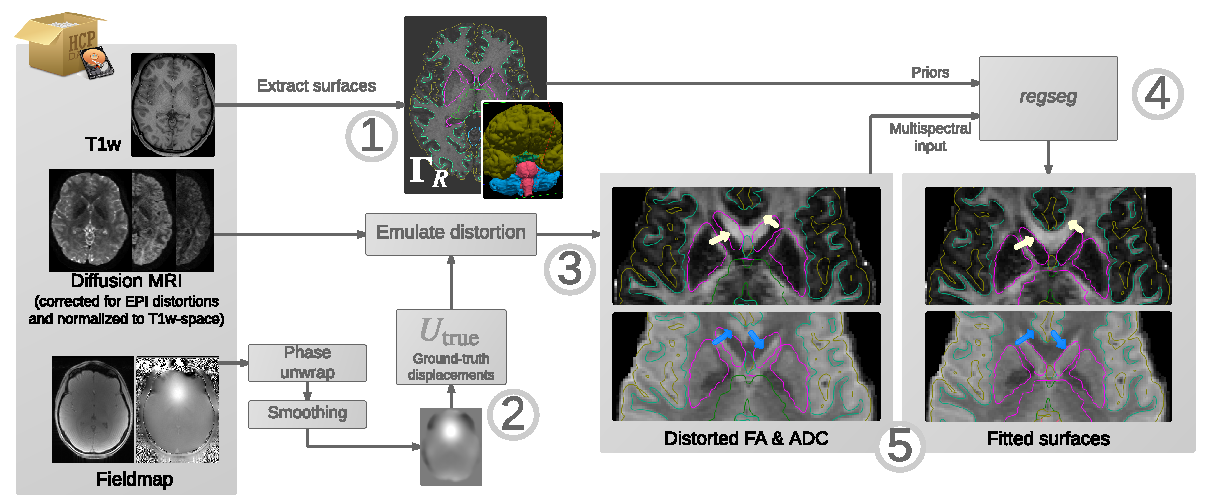
\includegraphics[width=\linewidth]{figures/figure04.pdf}
	\caption{Assessment of the segmentation model, sampling the value of the energy functional
	\eqref{eq:energy} versus several registration errors generated as explained in
	\nameref{sec:res_model_and_metric}.
	The metric of our registration method displayed a smooth gradient towards the minimum
	located at the $\epsilon = 0.0$ point.}\label{fig:energymap}
\end{figure}

\paragraph*{Evaluation \& cross-comparison}\label{sec:res_cc_evaluation}
%
Finally, we tested the performance of our registration method, and compared it to a competing
  method: the \emph{b0}-to-\gls*{t2} registration approach.
To this end, we integrated the registration software \emph{elastix} \citep{klein_elastix_2010},
  and reproduced the settings that internally uses \emph{ExploreDTI}
  \citep{leemans_exploredti_2009}, a widely used toolkit for tractography analysis of
  \gls*{dti}.
A dual workflow to the general evaluation framework (\autoref{fig:evworkflows})
  was also implemented to run the correction experiment with the competing method.
First, the average \emph{b0} volume is computed using all the \emph{low-b} volumes within
  the distorted \gls*{dmri} dataset.
Using the ``preprocessed'' instance of the \gls*{t2} image of the corresponding subject as
  reference image, and the \emph{b0} image as moving image, we registered both and
  projected the correct (undistorted) contours to the warped space using the resulting
  transform.
For both \emph{regseg} and the competing method, we computed the \gls*{swindex} \eqref{eq:swindex}
  of every surface.
Finally, to statistically compare the results from both methods we performed a one-way ANOVA test
  on the warping indices for three surfaces.
Following the nomenclature introduced in section \nameref{sec:human_connectome}, we selected
  $\Gamma_{VdGM}$, $\Gamma_{WM}$, and $\Gamma_{pial}$ as surfaces of interest.
These interfaces are critical in connectivity analyses, and small errors in their location may
  lead to discarding fundamental paths between regions.
We also reported the 95\% CIs of the warping indices for those surfaces.
The quantitative results of the ANOVA tests and the CIs are presented in \autoref{tab:results_real}.

\begin{table}
		\centering
		\footnotesize
		\tabcolsep=0.05cm
    \begin{tabular}{L{1.8cm}ccc}
                            & $\Gamma_{VdGM}$  & $\Gamma_{WM}$ & $\Gamma_{pial}$ \\
    \hline
    CI \emph{regseg}        & 0.39 - 0.64 & 0.64 - 0.83 & 0.76 - 0.93 \\
    CI competing            & 2.36 - 3.37 & 2.65 - 3.19 & 2.82 - 3.40 \\
    \hline
    ANOVA (f-stat/p-value)  & (51.81/1.5e-06) & (148.25/8.1e-10) & (143.01/1.1e-09) \\
    \hline
    \end{tabular}
    \caption{All the 95\% CIs of the \gls*{swindex} distributions computed for the
      surfaces of interest were lower for \emph{regseg} with respect to the competing
      method.
    CIs reported in this table were computed using bootstrapping with mean as location
      statistic and $10^4$ samples.
    One-way-ANOVA tests indicated that there is a significant difference between our method and
      the competing method of choice.
    }\label{tab:results_real}
\end{table}

\begin{figure*}
	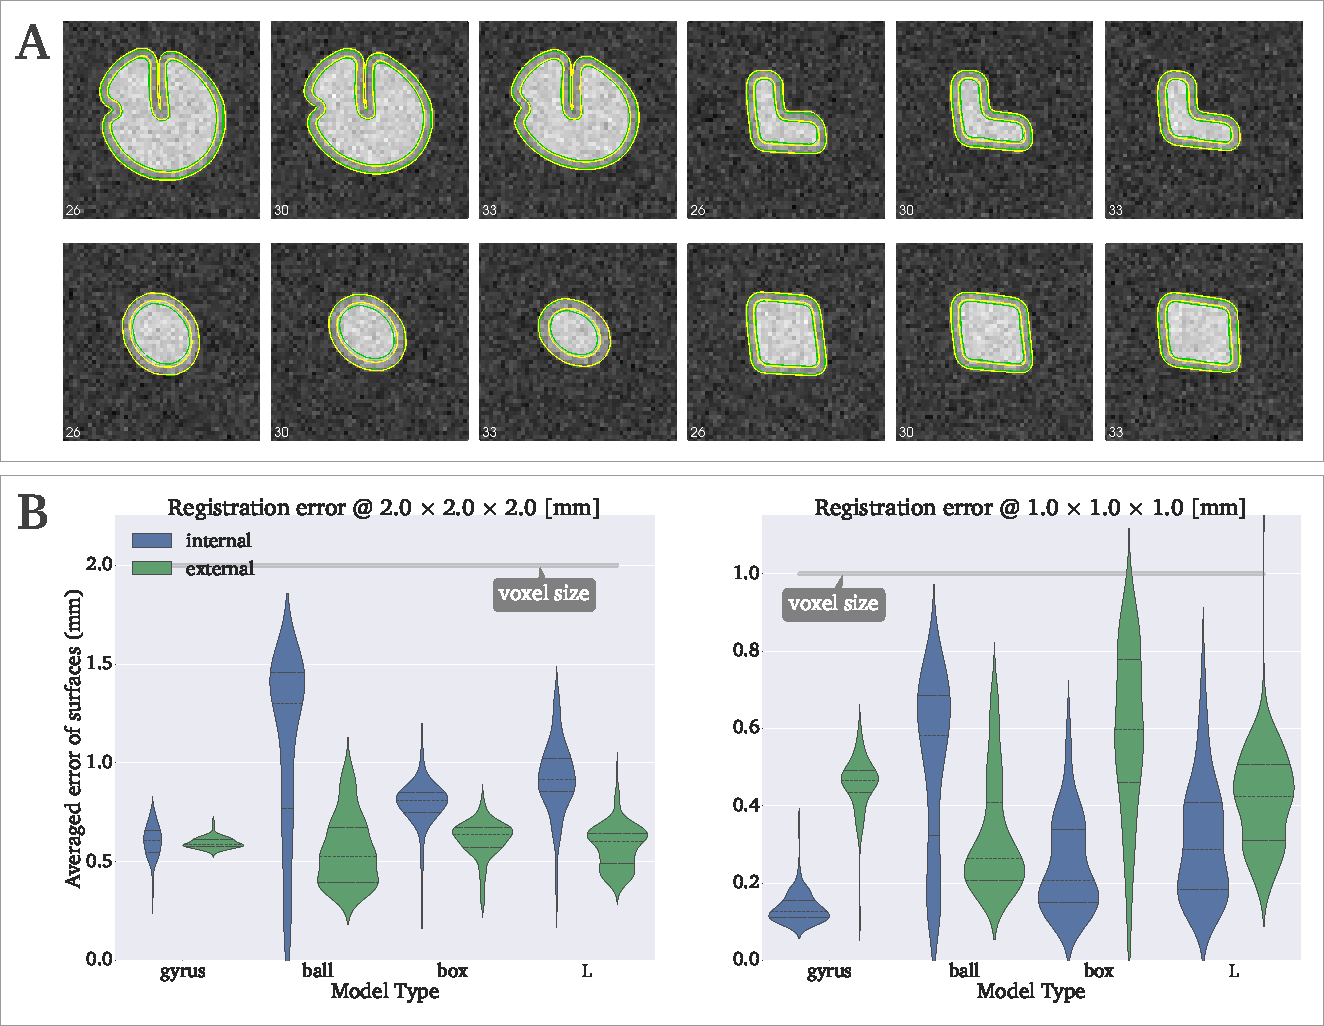
\includegraphics[width=\linewidth]{figures/figure05.pdf}
	\caption{The evaluation instrument automatically renders the overlay of the
	  target \gls*{fa} image and the resulting contours after distortion estimation (yellow color) and
	  their theoretical location using the ground-truth (green color).
	The first two rows show several axial slices for \emph{regseg} (``proposed'' row) and the
	  competing method.
	The last two rows represent the sagittal view.
	We intentionally omitted the coronal slicing due to it is the less informative given the properties
	  of the distortion.
	Red arrows point to regions where the accuracy of the proposed method more clearly overperformed
	  the competing method.
	\todo[inline]{This figure will also have the box-plots of the errors of surfaces for both regseg
	and the t2b method}
	}\label{fig:results_real}
\end{figure*}